% Report of the aco-tsp project.
%
% Build with:   latexmk -pdf report.tex        (or: cmake --build <dir> --target report)
%
% Every figure and table is drawn from the files in data/, which are produced
% by scripts/run-experiments.sh. Nothing in this document is a screenshot.

\documentclass[11pt,a4paper]{article}

% --- Fonts and page ----------------------------------------------------------
\usepackage[T1]{fontenc}
\usepackage[utf8]{inputenc}
\usepackage{newpxtext}
\usepackage[varbb]{newpxmath}
\usepackage[scaled=0.92]{inconsolata}
\usepackage[final]{microtype}
\usepackage[a4paper,margin=2.6cm,headheight=14pt]{geometry}
\linespread{1.06}

% --- Mathematics, tables, figures -------------------------------------------
\usepackage{amsmath}
\usepackage{booktabs}
\usepackage{array}
\usepackage{siunitx}
\usepackage{xcolor}
\usepackage{pgfplots}
\usepackage{tikz}
\usepackage{caption}
\usepackage{subcaption}
\usepackage{algorithm}
\usepackage{algpseudocode}
\usepackage{listings}
\usepackage{enumitem}
\usepackage{fancyhdr}
\usepackage[numbers,sort&compress]{natbib}
\usepackage[hidelinks]{hyperref}
\usepackage[capitalise,noabbrev]{cleveref}

\pgfplotsset{compat=1.18}
\usetikzlibrary{arrows.meta,backgrounds,positioning,fit}
\sisetup{group-separator={\,},group-minimum-digits=5}

% --- Colours and plot styles -------------------------------------------------
\definecolor{ink}{HTML}{111827}
\definecolor{rust}{HTML}{C2410C}
\definecolor{ocean}{HTML}{1D4ED8}
\definecolor{moss}{HTML}{15803D}
\definecolor{slate}{HTML}{6B7280}
\definecolor{mist}{HTML}{E5E7EB}
\definecolor{paper}{HTML}{F9FAFB}

\pgfplotsset{
  report/.style={
    width=\linewidth,
    height=5.4cm,
    grid=major,
    grid style={mist},
    axis lines=left,
    axis line style={slate},
    tick style={slate},
    tick label style={font=\footnotesize},
    label style={font=\small},
    legend style={font=\footnotesize,draw=mist,fill=white,legend cell align=left},
    every axis plot/.append style={line width=0.9pt},
  },
  sensitivity/.style={
    report,
    scale only axis,
    width=3.9cm,
    height=3.9cm,
  },
  tour/.style={
    scale only axis,
    width=0.9\linewidth,
    axis equal image,
    hide axis,
    xmin=-30,xmax=1030,ymin=-30,ymax=1030,
  },
}

% --- Listings ----------------------------------------------------------------
\lstdefinestyle{plain}{
  basicstyle=\ttfamily\footnotesize,
  backgroundcolor=\color{paper},
  frame=single,
  rulecolor=\color{mist},
  framesep=6pt,
  xleftmargin=8pt,
  xrightmargin=8pt,
  columns=fullflexible,
  keepspaces=true,
  showstringspaces=false,
  breaklines=true,
}
\lstdefinestyle{c}{
  style=plain,
  language=C,
  keywordstyle=\color{ocean},
  commentstyle=\color{slate}\itshape,
  stringstyle=\color{rust},
  morekeywords={size_t,bool,uint64_t,aco_instance,aco_tour,aco_error,aco_params,aco_colony,aco_iteration},
}
\lstset{style=plain}

% --- Headers -----------------------------------------------------------------
\pagestyle{fancy}
\fancyhf{}
\fancyhead[L]{\small\color{slate}Ant colony optimisation for the travelling salesman problem}
\fancyhead[R]{\small\color{slate}\thepage}
\renewcommand{\headrulewidth}{0.3pt}
\renewcommand{\headrule}{\color{mist}\hrule height \headrulewidth}

\setlist{itemsep=2pt,topsep=4pt}
\captionsetup{font=small,labelfont=bf,skip=6pt}

% --- Notation and generated numbers -----------------------------------------
\newcommand{\tool}{\texttt{aco-tsp}}
\newcommand{\code}[1]{\texttt{#1}}
\newcommand{\bigO}{\mathcal{O}}
\DeclareMathOperator*{\argmax}{arg\,max}
% A mean tour length, printed with one decimal.
\newcommand{\mean}[1]{\num[round-mode=places,round-precision=1]{#1}}

% Generated by scripts/run-experiments.sh -- do not edit.
\newcommand{\UniformNearestNeighbour}{9419}
\newcommand{\UniformTwoOpt}{8277}
\newcommand{\UniformAntSystemTour}{8517}
\newcommand{\UniformHybridTour}{8080}
\newcommand{\UniformAntSystemMean}{8442.00}
\newcommand{\UniformAntSystemBest}{8347}
\newcommand{\UniformElitistMean}{8239.15}
\newcommand{\UniformElitistBest}{8111}
\newcommand{\UniformHybridMean}{8068.35}
\newcommand{\UniformHybridBest}{8027}
\newcommand{\ExperimentRuns}{20}
\newcommand{\ExperimentIterations}{200}


% Generated table rows are read with the expandable primitive: a plain \input
% leaves tokens behind that break the \bottomrule which follows it.
\makeatletter
\newcommand{\inputrows}[1]{\@@input #1 }
\makeatother

\hypersetup{
  pdftitle={Solving the Travelling Salesman Problem with Ant Colony Optimisation},
  pdfauthor={Dmytro Palahin},
  pdfsubject={Design, implementation and evaluation of aco-tsp},
  pdfkeywords={ant colony optimisation, travelling salesman problem, metaheuristics, C},
}

\begin{document}

% =============================================================================
% Title page
% =============================================================================
\begin{titlepage}
  \centering
  \vspace*{2.2cm}

  {\small\scshape\color{slate} Project report\par}
  \vspace{1.1cm}

  {\Huge\bfseries\color{ink} Solving the Travelling Salesman\\[0.25em] Problem with Ant Colony\\[0.25em] Optimisation\par}
  \vspace{0.9cm}
  {\Large\color{slate} Design, implementation and evaluation of \tool\par}
  \vspace{1.6cm}

  \begin{tikzpicture}
    \begin{axis}[tour, width=7.4cm]
      \addplot[rust, line width=0.9pt] table[x index=0, y index=1] {data/tour_hybrid.dat};
      \addplot[only marks, mark=*, mark size=1.1pt, ink] table[x index=0, y index=1] {data/tour_hybrid.dat};
    \end{axis}
  \end{tikzpicture}
  \vspace{1.4cm}

  {\Large Dmytro Palahin\par}
  \vspace{0.5cm}
  {\normalsize Version 2.0 \quad$\cdot$\quad November 2026\par}

  \vfill
  \begin{minipage}{0.86\linewidth}
    \small\color{slate}\centering
    Revised and extended edition of a report written in February 2023, with a classmate,
    for the course \emph{Projet Informatique} (CP2I2, Sup Galilée, Université Sorbonne
    Paris Nord), taught by Frédéric Roupin.
  \end{minipage}
\end{titlepage}

% =============================================================================
\begin{abstract}
\noindent
This report describes \tool, a C11 library and command-line tool that searches for short
tours of the symmetric travelling salesman problem with ant colony optimisation. It states
the problem and the representation of its solutions, derives the Ant System algorithm and
three classic refinements, explains how they are implemented and verified, and evaluates
them experimentally. On \num{500} random instances small enough for the
optimum to be proven, Ant System finds it in \SIrange{89}{100}{\percent}
of the runs, and in every run once it is combined with a 2-opt local search. On the
instances of up to 100 cities supplied with the original assignment, that hybrid produces
tours \SIrange{2.9}{11.9}{\percent} shorter than a strong deterministic baseline, in about
half a second. The project started as second-year coursework; the report also documents
what was wrong with that first version and how the rewrite addresses it.
\end{abstract}

{\linespread{0.98}\selectfont\tableofcontents}
\clearpage

% =============================================================================
\section{Introduction}
\label{sec:introduction}
% =============================================================================

A delivery driver has $n$ customers to visit and wants to return home having driven as
little as possible. This is the \emph{travelling salesman problem} (TSP), one of the most
studied problems of combinatorial optimisation and one of the first shown to be
NP-hard~\cite{karp1972reducibility}: no algorithm is known that solves every instance in
time polynomial in $n$, and none is expected to exist. In practice one therefore settles for
\emph{heuristics}, which run fast and return good tours without any guarantee of
optimality.

\paragraph{Origin of the project.}
The work began in 2023 as the term project of the course \emph{Projet
Informatique}~\cite{roupin2023projet}. Each pair of students chose one of three problems
(DNA sequencing, delivery tours, scheduling with deadlines) and one of three generic
heuristics (simulated annealing, a genetic algorithm, an ant colony), and was asked to:
\begin{enumerate}[label=(\roman*)]
  \item state the function to optimise;
  \item choose a representation for the feasible solutions;
  \item specify the problem-dependent parts of the method, here how an ant moves and how
        the probability of a move is computed;
  \item implement the method in C and tune its parameters experimentally;
  \item evaluate and compare the results.
\end{enumerate}
We chose delivery tours and the ant colony. The program we handed in worked, in the sense
that it printed plausible tours, but it was a prototype: a single 300-line function,
hard-coded parameters, and several bugs that happened not to show on the instances we tried.

\paragraph{This edition.}
Three years later the program has been rewritten from scratch as a reusable library with a
test suite, and the evaluation, which in 2023 consisted of looking at pictures of tours, has
been redone quantitatively. The report follows the five items above:
\cref{sec:problem} covers (i) and (ii), \cref{sec:aco} covers (iii),
\cref{sec:implementation} covers the implementation, and \cref{sec:experiments} covers
the tuning and the evaluation. \Cref{sec:conclusion} concludes.

% =============================================================================
\section{The problem}
\label{sec:problem}
% =============================================================================

\subsection{Statement}

The customers and the depot are the vertices $1,\dots,n$ of a complete undirected graph.
The edge between $i$ and $j$ carries a weight $d_{ij}\ge 0$, the distance (or the travel
time) between the two places, with $d_{ij}=d_{ji}$ and $d_{ii}=0$. A \emph{tour} is a cycle
that visits every vertex exactly once, and the problem is to find a tour of minimum total
weight.

Nothing else is assumed about the distances. In particular they need not satisfy the
triangle inequality: the instances supplied with the assignment are matrices of arbitrary
integers. Instances built from points in the plane, where $d_{ij}$ is the Euclidean
distance, are an important special case and the only one that can be drawn.

\subsection{Objective function}

A tour is described by the order $\pi=(\pi_1,\dots,\pi_n)$ in which it visits the cities,
a permutation of $\{1,\dots,n\}$. Its length, the function to minimise, is
\begin{equation}
  L(\pi) \;=\; \sum_{i=1}^{n-1} d_{\pi_i\pi_{i+1}} \;+\; d_{\pi_n\pi_1},
  \label{eq:length}
\end{equation}
the last term being the trip back to the starting point. Rotating $\pi$ or reversing it
describes the same cycle, so there are $(n-1)!/2$ distinct tours: \num{181440}
for 10 cities, about $6\times 10^{16}$ for 20, and more than $10^{155}$ for 100. Enumeration
is hopeless beyond a dozen cities.

\subsection{Representation of a solution}

A tour is stored exactly as $\pi$: an array of $n$ city indices. This representation makes
every operation the algorithm needs cheap. Its length is computed in $\bigO(n)$ with
\cref{eq:length}; an ant extends a partial tour by appending one index; and the 2-opt move
of \cref{sec:local-search} is the reversal of a contiguous slice of the array.
\emph{Feasibility} is the condition that the array is a permutation, which the construction
procedure guarantees by never proposing a city twice. When a tour is printed it is rotated
to start at city~1, so that equal tours look equal.

The instance is stored as the full $n\times n$ matrix $(d_{ij})$ in one contiguous block,
row after row. Symmetry would allow half of it to be saved, but the matrix is read far
more often than anything else in the program, and $d_{ij}$ at offset $(i-1)n+(j-1)$ is one
multiplication away.

\subsection{Input format}

The assignment prescribes a text format: the number of cities, then the part of the
matrix above the diagonal, row by row. For five cities:

\begin{lstlisting}
5
61 789 204 349
362 135 376
260 45
880
\end{lstlisting}

\noindent
so that $d_{12}=61$, $d_{15}=349$ and $d_{45}=880$. The program also reads the common
subset of TSPLIB~\cite{reinelt1991tsplib}, the format of the standard benchmark library,
which can describe an instance by the coordinates of its cities.

% =============================================================================
\section{Ant colony optimisation}
\label{sec:aco}
% =============================================================================

\subsection{Principle}

Ants looking for food leave a chemical trail, a \emph{pheromone}, and tend to follow the
trails they come across. An ant that happens upon a short path to the food returns sooner,
so its trail is reinforced sooner and attracts more ants, who reinforce it further; trails
that are not maintained evaporate. No ant knows the terrain, yet the colony ends up using a
short path: the trails are a shared memory that the ants both read and write.

Ant colony optimisation~\cite{dorigo2004aco} turns this into an algorithm. Artificial ants
repeatedly build solutions step by step, at random, with a bias towards the choices that
earlier good solutions were made of. For the TSP a \emph{step} is a move from the current
city to one not visited yet, and the pheromone is a number $\tau_{ij}$ attached to every
edge. The first such algorithm, and the one implemented here, is \emph{Ant System}, due to
Dorigo, Maniezzo and Colorni~\cite{dorigo1996ant}.

\subsection{Ant System}
\label{sec:ant-system}

\paragraph{Moving an ant.}
The colony has $m$ ants. At each iteration every ant builds a complete tour. Suppose ant
$k$ stands in city $i$ and let $N_i^k$ be the set of cities it has not visited. It moves to
$j\in N_i^k$ with probability
\begin{equation}
  p_{ij}^{k} \;=\;
  \frac{\tau_{ij}^{\alpha}\,\eta_{ij}^{\beta}}
       {\displaystyle\sum_{l\in N_i^k}\tau_{il}^{\alpha}\,\eta_{il}^{\beta}},
  \qquad\text{where}\qquad \eta_{ij}=\frac{1}{d_{ij}}.
  \label{eq:transition}
\end{equation}
Two quantities make an edge attractive. Its \emph{visibility} $\eta_{ij}$ is fixed by the
instance and says that near cities are good candidates: it is the greedy part of the
decision. Its pheromone $\tau_{ij}$ changes over time and says that the edge belonged to
good tours: it is the experience of the colony. The exponents $\alpha$ and $\beta$ weigh one
against the other. With $\alpha=0$ the ants ignore each other and the algorithm is a
randomised greedy search; with $\beta=0$ they ignore the distances and can only amplify
whatever the first random tours contained.

In practice the choice is made by a \emph{roulette wheel}: the weights
$\tau_{il}^{\alpha}\eta_{il}^{\beta}$ of the candidates are laid end to end on a segment, a
point of the segment is drawn uniformly, and the candidate that owns it is selected.

\paragraph{Updating the pheromone.}
When all ants have completed their tours $T_1,\dots,T_m$, of lengths $L_1,\dots,L_m$, every
trail first loses a fraction $\rho$ of its pheromone and is then reinforced by the ants
that used it:
\begin{equation}
  \tau_{ij} \;\leftarrow\; (1-\rho)\,\tau_{ij} \;+\; \sum_{k=1}^{m}\Delta\tau_{ij}^{k},
  \qquad
  \Delta\tau_{ij}^{k} =
  \begin{cases}
    Q/L_k & \text{if the edge } \{i,j\} \text{ belongs to } T_k,\\
    0     & \text{otherwise.}
  \end{cases}
  \label{eq:update}
\end{equation}
An ant has a fixed budget $Q$ of pheromone and spreads it over its tour, so the edges of a
short tour receive more. Evaporation, governed by $\rho\in[0,1]$, is what lets the colony
forget: without it the first tours, which are essentially random, would weigh on the search
for ever.

\paragraph{Initialisation.}
The trails start from a common value $\tau_0$. If it is much smaller than the first
deposits, the first iteration decides everything; if it is much larger, many iterations
pass before the deposits matter. We follow the recommendation of Dorigo and
Stützle~\cite{dorigo2004aco} and set
\begin{equation}
  \tau_0 \;=\; \frac{m\,Q}{L_{\mathrm{nn}}},
  \label{eq:tau0}
\end{equation}
where $L_{\mathrm{nn}}$ is the length of a nearest-neighbour tour: this is the amount one
iteration would deposit on an edge if all ants followed that tour, that is, the order of
magnitude the trails will settle at. The 2023 program used the constant $\tau_0=0.2$, which
is far too large for instances with long distances and too small for instances with short
ones.

\Cref{alg:ant-system} summarises the method. Each ant starts from its own city when
$m=n$, as in the original paper, and from a random city otherwise.

\begin{algorithm}[htbp]
  \caption{Ant System for the travelling salesman problem}
  \label{alg:ant-system}
  \begin{algorithmic}[1]
    \Require distances $(d_{ij})$; parameters $m$, $\alpha$, $\beta$, $\rho$, $Q$; number of iterations $t_{\max}$
    \Ensure the best tour found, $T^{\ast}$
    \State $\tau_{ij}\gets\tau_0$ for every edge; \quad $L^{\ast}\gets\infty$
    \For{$t=1,\dots,t_{\max}$}
      \For{each ant $k=1,\dots,m$}
        \State place the ant in its starting city; mark every other city unvisited
        \While{some city is unvisited}
          \State choose the next city $j$ with the probabilities $p_{ij}^{k}$ of \cref{eq:transition}
          \State move to $j$ and mark it visited
        \EndWhile
        \State $L_k\gets$ length of the tour $T_k$ just built, back to the start included
        \State \textbf{if} $L_k<L^{\ast}$ \textbf{then} $T^{\ast}\gets T_k$; \; $L^{\ast}\gets L_k$
      \EndFor
      \State $\tau_{ij}\gets(1-\rho)\,\tau_{ij}$ for every edge \Comment{evaporation}
      \For{each ant $k$ and each edge $\{i,j\}$ of $T_k$}
        \State $\tau_{ij}\gets\tau_{ij}+Q/L_k$ \Comment{reinforcement}
      \EndFor
    \EndFor
    \State \Return $T^{\ast}$
  \end{algorithmic}
\end{algorithm}

\paragraph{Cost.}
An ant makes $n-1$ moves and examines the remaining cities at each of them, $n(n-1)/2$
candidates in total, so an iteration costs $\bigO(m\,n^2)$ for the construction and
$\bigO(n^2+m\,n)$ for the update. With one ant per city, the usual choice, this is
$\bigO(n^3)$ time per iteration and $\bigO(n^2)$ memory.

\subsection{Three refinements}
\label{sec:refinements}

Ant System was soon improved upon. The program implements three ideas from that later work;
each is off by default and can be enabled on its own.

\paragraph{Elitism.}
The best tour found so far, $T^{\ast}$, is reinforced at every iteration as if $e$
additional ants had followed it~\cite{dorigo1996ant}: the update~\eqref{eq:update} gains the
term $e\,Q/L^{\ast}$ on the edges of $T^{\ast}$. This focuses the search around the
incumbent and speeds up convergence, at the risk of converging too early.

\paragraph{Greedy exploitation.}
Ant Colony System~\cite{dorigo1997acs} replaces the roulette wheel by the
\emph{pseudo-random proportional rule}: with probability $q_0$ the ant goes straight to the
most attractive city, $j=\argmax_{l\in N_i^k}\tau_{il}^{\alpha}\eta_{il}^{\beta}$, and with
probability $1-q_0$ it draws from \cref{eq:transition} as before. Setting $q_0=1$
reproduces the first variant we tried in 2023, which always took the most probable city;
without randomness all ants soon follow the same tour, which is why we abandoned it.

\paragraph{Local search.}
\label{sec:local-search}
A tour built by an ant usually contains obvious defects, such as two edges that cross.
The 2-opt procedure~\cite{croes1958method} removes them: it looks for two edges
$\{a,b\}$ and $\{c,d\}$ of the tour such that
\[
  d_{ac}+d_{bd} \;<\; d_{ab}+d_{cd},
\]
replaces them by $\{a,c\}$ and $\{b,d\}$, which amounts to reversing the part of the tour
between $b$ and $c$, and repeats until no such pair exists. Applying it to every tour
before the pheromone update turns the colony into a guided multi-start local search: the
ants supply diverse, promising starting points and the trails remember which edges survive
the improvement. This combination is the main ingredient of the best-performing ant
algorithms for the TSP~\cite{stutzle2000mmas,dorigo2004aco}.

\subsection{Parameters}

\Cref{tab:parameters} lists the parameters, the options that set them and the defaults
retained after the study of \cref{sec:tuning}.

\begin{table}[htbp]
  \centering
  \caption{Parameters of the algorithm.}
  \label{tab:parameters}
  \begin{tabular}{@{}llll@{}}
    \toprule
    Symbol & Option & Default & Role \\
    \midrule
    $m$        & \code{-{}-ants}         & $n$                   & number of ants \\
    $t_{\max}$ & \code{-{}-iterations}   & 200                   & number of iterations \\
    $\alpha$   & \code{-{}-alpha}        & 1                     & weight of the pheromone \\
    $\beta$    & \code{-{}-beta}         & 3                     & weight of the visibility \\
    $\rho$     & \code{-{}-rho}          & 0.5                   & evaporation rate \\
    $Q$        & \code{-{}-deposit}      & 1                     & pheromone budget of an ant \\
    $\tau_0$   & \code{-{}-tau0}         & $mQ/L_{\mathrm{nn}}$  & initial pheromone \\
    $e$        & \code{-{}-elitist}      & 0                     & weight of the best-so-far tour \\
    $q_0$      & \code{-{}-q0}           & 0                     & probability of a greedy move \\
               & \code{-{}-local-search} & none                  & \code{none} or \code{2opt} \\
               & \code{-{}-patience}     & off                   & iterations without progress before stopping \\
    \bottomrule
  \end{tabular}
\end{table}

% =============================================================================
\section{Implementation}
\label{sec:implementation}
% =============================================================================

\subsection{Architecture}

The code is a static library, \code{libaco}, and a command-line tool, \tool, that is a
thin layer on top of it. \Cref{fig:architecture} shows the modules and their
dependencies, which form a hierarchy without cycles. The library is written in standard
C11 and depends on nothing but the C library. It is developed with GCC and Clang, and
avoids every construct that would prevent it from building with MSVC.

\begin{figure}[htbp]
  \centering
  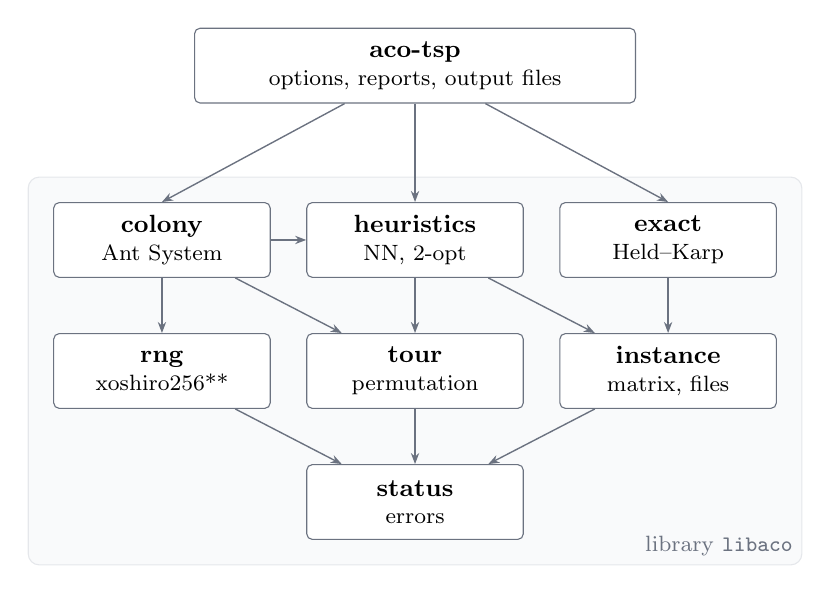
\begin{tikzpicture}[
      module/.style={draw=slate, rounded corners=2pt, fill=white, minimum height=0.95cm,
                     minimum width=2.75cm, align=center, font=\small},
      dependency/.style={-{Stealth[length=4pt]}, slate, line width=0.5pt},
      layer/.style={draw=mist, fill=paper, rounded corners=4pt, inner sep=9pt},
      node distance=0.7cm and 0.45cm,
    ]
    \node[module] (colony) {\textbf{colony}\\[-1pt]\footnotesize Ant System};
    \node[module, right=of colony] (heuristics) {\textbf{heuristics}\\[-1pt]\footnotesize NN, 2-opt};
    \node[module, right=of heuristics] (exact) {\textbf{exact}\\[-1pt]\footnotesize Held--Karp};
    \node[module, below=of colony] (rng) {\textbf{rng}\\[-1pt]\footnotesize xoshiro256**};
    \node[module, right=of rng] (tour) {\textbf{tour}\\[-1pt]\footnotesize permutation};
    \node[module, right=of tour] (instance) {\textbf{instance}\\[-1pt]\footnotesize matrix, files};
    \node[module, below=of tour] (status) {\textbf{status}\\[-1pt]\footnotesize errors};
    \node[module, above=1.25cm of heuristics, minimum width=5.6cm] (cli) {\textbf{aco-tsp}\\[-1pt]\footnotesize options, reports, output files};
    \begin{scope}[on background layer]
      \node[layer, fit=(colony)(exact)(rng)(instance)(status)] (library) {};
    \end{scope}
    \node[font=\footnotesize\color{slate}, anchor=south east] at (library.south east) {library \code{libaco}};
    \draw[dependency] (cli) -- (colony.north);
    \draw[dependency] (cli) -- (heuristics);
    \draw[dependency] (cli) -- (exact.north);
    \draw[dependency] (colony) -- (heuristics);
    \draw[dependency] (colony) -- (rng);
    \draw[dependency] (colony) -- (tour);
    \draw[dependency] (heuristics) -- (tour);
    \draw[dependency] (heuristics) -- (instance);
    \draw[dependency] (exact) -- (instance);
    \draw[dependency] (rng) -- (status);
    \draw[dependency] (tour) -- (status);
    \draw[dependency] (instance) -- (status);
  \end{tikzpicture}
  \caption{Modules and their main dependencies. An arrow from $A$ to $B$ means that $A$ uses $B$.}
  \label{fig:architecture}
\end{figure}

Two kinds of types appear in the interface. An instance and a colony are \emph{opaque
handles}: they can only be created by functions that validate their input, so the rest of
the code can rely on a square, symmetric, finite, non-negative matrix with a zero diagonal
without checking it again. Tours, parameters and statistics are plain structures. Every
function that can fail returns a status code and, where an explanation is useful, fills in
a message; the library never prints and never terminates the program. A complete use of the
library is short:

\begin{lstlisting}[style=c]
aco_instance *instance = NULL;
aco_tour tour = ACO_TOUR_INIT;
aco_error error = ACO_ERROR_INIT;
aco_params params = aco_params_default();

params.local_search = ACO_LOCAL_SEARCH_TWO_OPT;
params.seed = 42;

if (aco_instance_load("cities.tsp", &instance, &error) == ACO_OK &&
    aco_solve(instance, &params, &tour, &error) == ACO_OK) {
    printf("best tour: %g\n", tour.length);
} else {
    fprintf(stderr, "error: %s\n", error.message);
}
aco_tour_free(&tour);
aco_instance_destroy(instance);
\end{lstlisting}

\subsection{The inner loop}

Almost all the running time is spent choosing the next city of an ant, so three decisions
there matter.

\begin{description}[leftmargin=0pt]
  \item[Attractiveness is tabulated.] The product $\tau_{ij}^{\alpha}\eta_{ij}^{\beta}$ of
    \cref{eq:transition} does not change while the ants of one iteration are moving. It is
    computed once per iteration for all edges, and $\eta_{ij}^{\beta}$ once per run. A
    decision then costs additions and comparisons only; the 2023 code called \code{pow}
    twice for every candidate of every decision.
  \item[Unvisited cities are kept in a compact array.] Visiting a city removes it by
    moving the last element of the array into its place, in constant time, so a decision
    only looks at cities that are still candidates. The 2023 code searched the partial
    route to find out whether a city had been visited, which made the construction of a
    single tour cubic in $n$.
  \item[Nothing is allocated.] The colony allocates its buffers when it is created and
    reuses them at every iteration.
\end{description}

\subsection{Numerical robustness}

The formulas hide a few traps, which the implementation handles explicitly.

\begin{itemize}
  \item The visibility is measured in units of the shortest positive distance of the
    instance, $\eta_{ij}=d_{\min}/d_{ij}\in(0,1]$. Only ratios matter in
    \cref{eq:transition}, and bounded values cannot overflow when raised to a large
    power~$\beta$.
  \item Two cities at the same place have $d_{ij}=0$. They receive the largest visibility
    instead of a division by zero.
  \item With extreme parameters every weight of a decision can underflow to zero. The ant
    then chooses uniformly among the candidates rather than dividing by a zero sum.
  \item In floating-point arithmetic two tours can each appear shorter than the other by a
    rounding error, and 2-opt could alternate between them for ever. A move is accepted
    only if it shortens the tour by more than a tiny fraction of the edges it removes.
\end{itemize}

\subsection{Randomness and reproducibility}

The roulette wheel of the 2023 program drew its point with \code{rand() \% 100}, so the
wheel had only a hundred positions. A candidate whose slice contained none of them could
never be selected, and on an instance of 100 cities, where the average probability of a
candidate is \SI{1}{\percent}, that is the fate of many. The generator was also never
seeded, and its sequence differs from one C library to another.

The library carries its own generator, xoshiro256**~\cite{blackman2021scrambled}, seeded
through SplitMix64. It is fast, passes the standard statistical tests, has an explicit
state, so two colonies never disturb each other, and produces the same sequence on every
platform. A run is therefore a deterministic function of the instance, the parameters and
the seed, which makes results reproducible and failures debuggable.

\subsection{Reference solvers}

To judge the colony one needs something to compare it with. The library provides three
solvers for that purpose.

\begin{description}[leftmargin=0pt]
  \item[Nearest neighbour.] From a starting city, go to the closest unvisited city until
    none is left~\cite{rosenkrantz1977analysis}. It is the simplest reasonable heuristic,
    runs in $\bigO(n^2)$, and also provides the length $L_{\mathrm{nn}}$ of
    \cref{eq:tau0}.
  \item[Nearest neighbour followed by 2-opt.] The local search of
    \cref{sec:local-search} applied to a greedy tour: a much stronger baseline.
  \item[Exact dynamic programming.] The algorithm of Held and
    Karp~\cite{held1962dynamic} computes, for every set $S$ of cities and every $j\in S$,
    the length $C(S,j)$ of the shortest path that leaves city~1, visits exactly $S$ and
    ends in $j$:
    \[
      C(\{j\},j)=d_{1j},\qquad
      C(S,j)=\min_{k\in S\setminus\{j\}}\bigl(C(S\setminus\{j\},k)+d_{kj}\bigr).
    \]
    The optimum is $\min_j C(\{2,\dots,n\},j)+d_{j1}$. With $\bigO(n^2 2^n)$ time and
    $\bigO(n\,2^n)$ memory it is limited to 20 cities, where it takes a quarter of a
    second, but within that limit it provides the ground truth against which the heuristics
    are tested.
\end{description}

When used as baselines in \cref{sec:experiments}, the two heuristics are run from each
of the $n$ possible starting cities and the best tour is kept, which gives them a budget
comparable to one iteration of a colony with $n$ ants.

\subsection{From the 2023 prototype to version 2}

\Cref{tab:rewrite} lists the defects of the original program and what replaced them.
The first is the most serious: every array of $N$ elements was indexed from 1 to $N$, so
the program wrote past the end of each of them. It only appeared to work because the
overwritten memory usually belonged to a neighbouring array.

\begin{table}[htbp]
  \centering
  \caption{Defects of the 2023 program and their remedy in version 2.}
  \label{tab:rewrite}
  \small
  \begin{tabular}{@{}p{0.47\linewidth}p{0.48\linewidth}@{}}
    \toprule
    2023 prototype & Version 2 \\
    \midrule
    Arrays of $N$ elements indexed from 1 to $N$: out-of-bounds reads and writes
      & Zero-based indexing; whole test suite run under AddressSanitizer and Valgrind \\[3pt]
    Matrices in variable-length arrays on the stack: the instance size is limited by the stack
      & One heap block per matrix, allocated once and checked \\[3pt]
    Roulette wheel drawn with \code{rand() \% 100}; generator not seeded
      & 53-bit uniform draws from a seeded, portable generator \\[3pt]
    Membership test by scanning the route: $\bigO(n^3)$ per ant
      & Compact array of unvisited cities: $\bigO(n^2)$ per ant \\[3pt]
    Instance, parameters and output files fixed at compile time
      & Command-line options; nothing to recompile \\[3pt]
    Input files neither checked for existence nor validated
      & Parser with line-numbered diagnostics, fuzzed \\[3pt]
    Four copies of the same \code{main} function (1600 lines in total)
      & A library of independent modules, each with its tests \\[3pt]
    Plot through a pipe to a hard-coded Windows path
      & Portable data files and gnuplot scripts \\
    \bottomrule
  \end{tabular}
\end{table}

\subsection{Verification}

A program that returns \emph{a} tour is easy to write and hard to trust, since a wrong
answer looks just like a mediocre one. The project therefore invests in several
independent layers of verification.

\begin{itemize}
  \item \textbf{Unit tests} (73, in five programs) exercise each module through its public
    interface, including the error paths. The exact solver is checked against brute-force
    enumeration; 2-opt is checked on points placed on a circle, where the optimum is the
    perimeter of a regular polygon; one iteration of the pheromone update is checked
    against the value of \cref{eq:update} computed by hand.
  \item \textbf{Properties of the search} are tested rather than particular outputs: the
    same seed gives the same run, the best tour never gets worse, the trails stay
    symmetric and positive, and on small instances the result stays within a stated margin
    of the proven optimum.
  \item \textbf{End-to-end tests} (44 checks) run the command-line tool and verify its
    exit status, its messages and the files it writes.
  \item \textbf{Fuzzing.} The parser is the only code that reads untrusted data. A
    libFuzzer harness feeds it mutated files under AddressSanitizer and
    UndefinedBehaviorSanitizer; several million inputs are tried on every push.
  \item \textbf{Analysis.} The code compiles without warnings under a strict warning set
    with GCC and Clang, and passes clang-tidy with every finding treated as an error.
\end{itemize}

The tests cover \SI{93.6}{\percent} of the lines and every function of the library and of
the tool; what remains is almost entirely the handling of failed memory allocations. A
continuous-integration pipeline repeats all of this for every change on Linux, macOS and
Windows, and adds a CodeQL analysis.

% =============================================================================
\section{Experiments}
\label{sec:experiments}
% =============================================================================

\subsection{Protocol}

Unless stated otherwise the colony has one ant per city and runs for
\ExperimentIterations{} iterations with the default parameters of
\cref{tab:parameters}. Because the algorithm is randomised, every configuration is run
with \ExperimentRuns{} different seeds and we report the mean length, the standard
deviation and the best run. Three variants are compared: plain Ant System (AS), elitist
Ant System with $e=n$, and Ant System with 2-opt.

Two families of instances are used: the seven matrices supplied with the assignment, of 5
to 100 cities, whose distances are arbitrary integers; and random Euclidean instances,
generated by the program itself, with integer coordinates drawn uniformly from
$[0,1000]^2$ and distances rounded to the nearest integer. One of the latter, with 100
cities, serves for the tuning and the illustrations.

Times were measured on a laptop with an Apple M1~Pro processor, the program being compiled
with Apple Clang~21 at \code{-O3} and running on a single core. All the data of this
section can be regenerated with \code{scripts/run-experiments.sh}; the tour lengths are
identical from one machine to another, only the timings change.

\subsection{Validation against proven optima}
\label{sec:validation}

The first question is whether the algorithm finds optimal tours when they are known.
For each size from 8 to 16 cities we generated 100 random Euclidean instances, computed
their optimum with the exact solver, and ran each variant once. \Cref{tab:exact} gives
the proportion of instances solved to optimality and the relative excess over the optimum.

\begin{table}[htbp]
  \centering
  \caption{Small random instances: frequency of reaching the proven optimum, and excess
    length over it.}
  \label{tab:exact}
  \begin{tabular}{@{}rrrrrrr@{}}
    \toprule
    & & \multicolumn{3}{c}{Ant System} & \multicolumn{2}{c}{Ant System + 2-opt} \\
    \cmidrule(lr){3-5}\cmidrule(l){6-7}
    Cities & Instances & Optimal & Mean excess & Worst excess & Optimal & Mean excess \\
    \midrule
    \inputrows{data/exact_rows.tex}
    \bottomrule
  \end{tabular}
\end{table}

Plain Ant System reaches the optimum in about nine runs out of ten and is on average
within \SI{0.15}{\percent} of it, although an unlucky run can end
\SI{5}{\percent} to \SI{6}{\percent} above. With 2-opt, all 500 runs returned an optimal
tour. Beyond their intrinsic interest, these figures are strong evidence that the
implementation is correct.

\subsection{Tuning the parameters}
\label{sec:tuning}

\Cref{fig:sensitivity} shows the effect of $\alpha$, $\beta$ and $\rho$ on plain Ant
System, each varied alone around the default configuration, on the random instance of 100
cities.

\begin{figure}[htbp]
  \centering
  \begin{subfigure}{0.40\linewidth}
    \raggedleft
    \begin{tikzpicture}
      \begin{axis}[sensitivity, xlabel={$\alpha$}, ylabel={mean tour length},
                   ymin=8300, ymax=9700, xmin=0.3, xmax=4.2, xtick={0.5,1,2,3,4},
                   scaled y ticks=false, yticklabel style={/pgf/number format/fixed, /pgf/number format/1000 sep={\,}}]
        \addplot[rust, mark=*, mark size=1.4pt, error bars/.cd, y dir=both, y explicit]
          table[x index=0, y index=1, y error index=2] {data/sensitivity_alpha.dat};
      \end{axis}
    \end{tikzpicture}
  \end{subfigure}\hfill
  \begin{subfigure}{0.29\linewidth}
    \centering
    \begin{tikzpicture}
      \begin{axis}[sensitivity, xlabel={$\beta$},
                   ymin=8300, ymax=9700, xmin=0.5, xmax=10.5, xtick={1,2,4,6,8,10},
                   yticklabels={}]
        \addplot[ocean, mark=*, mark size=1.4pt, error bars/.cd, y dir=both, y explicit]
          table[x index=0, y index=1, y error index=2] {data/sensitivity_beta.dat};
      \end{axis}
    \end{tikzpicture}
  \end{subfigure}\hfill
  \begin{subfigure}{0.29\linewidth}
    \centering
    \begin{tikzpicture}
      \begin{axis}[sensitivity, xlabel={$\rho$},
                   ymin=8300, ymax=9700, xmin=-0.04, xmax=1.04, xtick={0,0.25,0.5,0.75,1},
                   yticklabels={}]
        \addplot[moss, mark=*, mark size=1.4pt, error bars/.cd, y dir=both, y explicit]
          table[x index=0, y index=1, y error index=2] {data/sensitivity_rho.dat};
      \end{axis}
    \end{tikzpicture}
  \end{subfigure}
  \caption{Sensitivity of Ant System to its three main parameters on 100 random cities.
    Each point is the mean of \ExperimentRuns{} runs and the bars show one standard
    deviation. The points $\alpha=0$ (mean \num{12123}) and $\beta=0$
    (mean \num{41867}) lie far above the frame.}
  \label{fig:sensitivity}
\end{figure}

\begin{description}[leftmargin=0pt]
  \item[Both sources of information are necessary.] Without pheromone ($\alpha=0$) the
    mean tour is \SI{44}{\percent} longer than with $\alpha=1$; without
    visibility ($\beta=0$) it is five times longer, barely better than a random tour. The
    greedy information matters most, but it is the pheromone that turns a randomised greedy
    search into an optimiser.
  \item[$\alpha=1$ is the best value.] Larger values make the ants follow the trails too
    faithfully: the mean degrades and, tellingly, the spread between runs doubles, the sign
    of a search that locks onto whichever tour came first.
  \item[$\beta$ has a broad optimum between 2 and 5.] The original program used $\beta=1$
    in one of its versions, which costs \SI{16}{\percent} here.
  \item[$\rho$ hardly matters above 0.1.] Differences in that range are of the order of
    the noise. Very slow evaporation ($\rho\le 0.05$) costs one to two percent with a
    budget of 200 iterations: the early, poor tours are forgotten too slowly.
\end{description}

We retain $\alpha=1$, $\beta=3$ and $\rho=0.5$, which agree with the values recommended in
the literature~\cite{dorigo2004aco}.

\subsection{Results on the instances of the assignment}

\begin{table}[htbp]
  \centering
  \caption{Tour lengths on the instances of the assignment. The baselines keep the best of
    $n$ starting cities; the colony columns give the mean and the best of
    \ExperimentRuns{} runs of \ExperimentIterations{} iterations. The optimum is known
    for the first three instances only.}
  \label{tab:course}
  \small
  \setlength{\tabcolsep}{5pt}
  \begin{tabular}{@{}lrr rr rr rr rr@{}}
    \toprule
    & & & \multicolumn{2}{c}{Baselines} & \multicolumn{2}{c}{Ant System}
        & \multicolumn{2}{c}{Elitist AS} & \multicolumn{2}{c}{AS + 2-opt} \\
    \cmidrule(lr){4-5}\cmidrule(lr){6-7}\cmidrule(lr){8-9}\cmidrule(l){10-11}
    Instance & $n$ & Optimum & NN & NN + 2-opt & mean & best & mean & best & mean & best \\
    \midrule
    \inputrows{data/course_rows.tex}
    \bottomrule
  \end{tabular}
\end{table}

\Cref{tab:course} compares the three variants with the two baselines. Four observations
can be made.

\begin{enumerate}
  \item \textbf{The small instances are solved.} For 5, 10 and 20 cities the optimum is
    known; every variant finds it on the first two, and on \code{tsp020} the hybrid finds
    it in all \ExperimentRuns{} runs while plain Ant System does so in its best run.
  \item \textbf{Ant System clearly beats the greedy heuristic}, by
    \SIrange{13}{23}{\percent}, which is what the 2023 report observed
    qualitatively.
  \item \textbf{Plain Ant System does not beat a good local search.} Nearest neighbour
    followed by 2-opt, restarted from every city, does as well or better on every instance,
    and does so in a few milliseconds. This sobering comparison is absent from the original
    report, which had no baseline at all. Elitism narrows the gap and overtakes the
    baseline on three of the five larger instances, including the two largest, where
    focusing the search pays off.
  \item \textbf{The hybrid is the best method on every instance.} From 20 cities upwards
    its mean tour is \SIrange{2.9}{11.9}{\percent} shorter than the stronger baseline, and
    it is also the most stable, its standard deviation being several times smaller than
    that of Ant System. The ants and the local search complement each other. The price is
    time: about half a second for 100 cities, where the baseline needs three milliseconds
    and plain Ant System \SI{0.15}{\second}.
\end{enumerate}

\subsection{Convergence}

\begin{figure}[htbp]
  \centering
  \begin{tikzpicture}
    \begin{axis}[report, height=6.4cm, width=0.92\linewidth,
                 xlabel={iteration}, ylabel={best tour length so far (mean of \ExperimentRuns{} runs)},
                 xmin=0, xmax=200, ymin=7900, ymax=10400,
                 scaled y ticks=false,
                 yticklabel style={/pgf/number format/fixed, /pgf/number format/1000 sep={\,}},
                 legend pos=north east]
      \addplot[rust] table[x index=0, y index=1] {data/convergence.dat};
      \addlegendentry{Ant System}
      \addplot[ocean] table[x index=0, y index=2] {data/convergence.dat};
      \addlegendentry{Elitist Ant System}
      \addplot[moss] table[x index=0, y index=3] {data/convergence.dat};
      \addlegendentry{Ant System + 2-opt}
      \addplot[slate, dashed, line width=0.6pt, domain=0:200, samples=2] {\UniformNearestNeighbour};
      \addlegendentry{nearest neighbour}
      \addplot[slate, densely dotted, line width=0.8pt, domain=0:200, samples=2] {\UniformTwoOpt};
      \addlegendentry{nearest neighbour + 2-opt}
    \end{axis}
  \end{tikzpicture}
  \caption{Convergence on 100 random cities. The first iterations of the two variants
    without local search, above \num{13000}, are cut off.}
  \label{fig:convergence}
\end{figure}

\Cref{fig:convergence} follows the best tour found so far on the random instance. Plain
Ant System improves quickly during the first thirty iterations, when the trails take
shape, and slowly afterwards; it ends at \mean{\UniformAntSystemMean} on average, well below
the greedy tour (\num{\UniformNearestNeighbour}) but above the
local-search baseline (\num{\UniformTwoOpt}). The elitist variant
converges faster and lower, to \mean{\UniformElitistMean}, just under that baseline. The
hybrid is of another kind: its very first iteration, which is nothing but 100 randomised
greedy tours improved by 2-opt, is already better than the final result of plain Ant
System, and the trails then guide it down to \mean{\UniformHybridMean}. All three curves flatten well
before the end, which indicates that 200 iterations are sufficient at this size and that
additional effort would be better spent on diversification than on more iterations.

\Cref{fig:tours} shows what the numbers mean geometrically. The greedy tour is
recognisable by the long edges it needs at the end to collect the cities it left behind;
the tour of the hybrid has no crossing and no detour of that kind.

\begin{figure}[htbp]
  \centering
  \begin{subfigure}{0.48\linewidth}
    \centering
    \begin{tikzpicture}
      \begin{axis}[tour]
        \addplot[slate, line width=0.8pt] table[x index=0, y index=1] {data/tour_nearest_neighbour.dat};
        \addplot[only marks, mark=*, mark size=1pt, ink] table[x index=0, y index=1] {data/tour_nearest_neighbour.dat};
      \end{axis}
    \end{tikzpicture}
    \caption{Nearest neighbour: \num{\UniformNearestNeighbour}}
  \end{subfigure}\hfill
  \begin{subfigure}{0.48\linewidth}
    \centering
    \begin{tikzpicture}
      \begin{axis}[tour]
        \addplot[rust, line width=0.8pt] table[x index=0, y index=1] {data/tour_hybrid.dat};
        \addplot[only marks, mark=*, mark size=1pt, ink] table[x index=0, y index=1] {data/tour_hybrid.dat};
      \end{axis}
    \end{tikzpicture}
    \caption{Ant System + 2-opt: \num{\UniformHybridTour}}
  \end{subfigure}
  \caption{Two tours of the same 100 random cities.}
  \label{fig:tours}
\end{figure}

\subsection{Running time}

\begin{figure}[htbp]
  \centering
  \begin{tikzpicture}
    \begin{loglogaxis}[report, height=5.8cm, width=0.62\linewidth,
                       xlabel={number of cities $n$}, ylabel={seconds per iteration},
                       xmin=20, xmax=1000, ymin=4e-6, ymax=1,
                       xtick={25,50,100,200,400,800}, xticklabels={25,50,100,200,400,800},
                       ytick={1e-5,1e-4,1e-3,1e-2,1e-1,1},
                       minor tick style={draw=none},
                       legend pos=north west]
      \addplot[rust, only marks, mark=*, mark size=2pt] table[x index=0, y index=2] {data/scaling.dat};
      \addlegendentry{measured}
      \addplot[slate, dashed, line width=0.6pt, domain=20:1000, samples=2] {7.26e-10*x^3};
      \addlegendentry{$c\,n^3$}
    \end{loglogaxis}
  \end{tikzpicture}
  \caption{Time of one iteration of Ant System with one ant per city.}
  \label{fig:scaling}
\end{figure}

\Cref{fig:scaling} plots the time of one iteration against the size of the instance, with
$m=n$. On logarithmic axes the measurements fall on a line of slope 3, as the analysis of
\cref{sec:ant-system} predicts: doubling the number of cities multiplies the time by
eight. In absolute terms an iteration takes \SI{0.72}{\milli\second}
for 100 cities and \SI{0.37}{\second} for 800, so the default 200
iterations take \SI{0.15}{\second} and about 75 seconds respectively.
The local search multiplies these times by about four at 100 cities. The cubic growth is
the practical limit of the method as implemented: instances of several thousand cities
would require the candidate lists discussed below.

% =============================================================================
\section{Conclusion}
\label{sec:conclusion}
% =============================================================================

The five tasks of the assignment have been carried out. The objective is the length of a
closed tour, a solution is a permutation, an ant moves according to the random proportional
rule and the colony learns through evaporation and reinforcement. The algorithm is
implemented as a tested C library, its parameters have been tuned by experiment, and its
results have been compared with two heuristics and with an exact method.

The experiments support three conclusions. First, the implementation can be trusted: it
finds proven optima on small instances. Second, the parameters behave as the literature
describes, and the defaults $\alpha=1$, $\beta=3$, $\rho=0.5$ are sound. Third, and less
expected by the students we were in 2023, Ant System alone is not competitive with a
simple local search; its value appears when the two are combined, the hybrid being the
best method on every instance we tried.

The exercise of rewriting the program was instructive in its own right. Most of the
defects of the first version were invisible in its output, and were found only because the
new version was built to be checked: by tests, by sanitizers, by a fuzzer, and by baselines
that could contradict us.

\paragraph{Further work.}
Several extensions follow directly from the limits observed.
\emph{Candidate lists}, which restrict each decision to the nearest few cities, would cut
the cost of an iteration from $\bigO(n^3)$ to $\bigO(n^2)$ and open the way to much larger
instances. \emph{MAX--MIN Ant System}~\cite{stutzle2000mmas}, which bounds the trails and
lets only the best ant deposit, addresses the premature convergence visible in
\cref{fig:convergence}. The ants of one iteration are independent and could build their
tours \emph{in parallel}. Finally, the delivery problem of the assignment mentions time
windows for the customers, which would turn the construction step into a constrained one.

\phantomsection
\addcontentsline{toc}{section}{References}
\bibliographystyle{unsrtnat}
\bibliography{references}

% =============================================================================
\clearpage
\appendix
\section{Using the program}
\label{sec:usage}
% =============================================================================

The program is built with CMake and has no dependency:

\begin{lstlisting}
cmake --workflow --preset release
\end{lstlisting}

\noindent
This configures the project, compiles it and runs the tests. A typical session then looks
as follows.

\begin{lstlisting}
$ build/release/aco-tsp solve data/random/random100.tsp --seed 1 --local-search 2opt
instance     random100 (100 cities)
algorithm    ant colony optimisation
parameters   ants=100 iterations=200 alpha=1 beta=3 rho=0.5 deposit=1
             tau0=0.009882 q0=0 elitist=0 local-search=2opt
seed         1
iterations   200 (best tour found at iteration 55)
time         0.582 s
length       8080
tour         1 2 58 54 12 4 38 13 18 78 80 26 39 77 69 81 65 53 64 84 15 74 9
             ...
\end{lstlisting}

\noindent
Other useful invocations:

\begin{lstlisting}
# Baselines and the exact solver
aco-tsp solve data/course/tsp020.txt --algorithm nearest-neighbour
aco-tsp solve data/course/tsp020.txt --algorithm two-opt
aco-tsp solve data/course/tsp020.txt --algorithm exact

# A new random instance, solved, with files for plotting
aco-tsp generate --cities 200 --seed 3 --output cities.tsp
aco-tsp solve cities.tsp --elitist 200 --plot tour.dat --trace trace.csv
gnuplot -e "input='tour.dat'; output='tour.svg'" scripts/plot-tour.gp

# Regenerate the data of every table and figure of this report
scripts/run-experiments.sh build/release/aco-tsp
\end{lstlisting}

\noindent
The complete list of options is printed by \code{aco-tsp help solve}; the file formats are
specified in \code{docs/file-formats.md} and the organisation of the code in
\code{docs/architecture.md}.

\end{document}
